\documentclass[./bab_3.tex]{subfiles}
\begin{document}
\section{Analisis dan Rancangan Sistem}
\begin{figure}[ht!]
  \begin{center}
    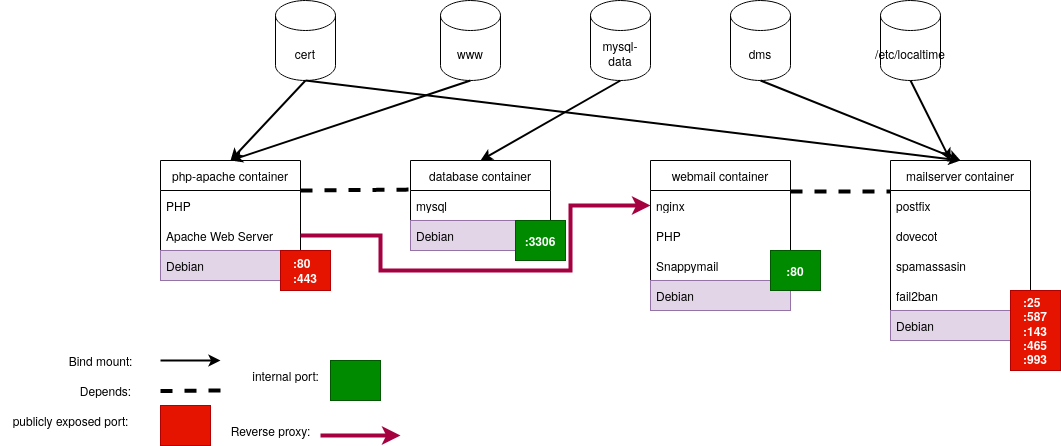
\includegraphics[width=0.95\textwidth]{desain.png}
  \end{center}
  \caption{Rancangan susunan docker \textit{container}}
  \label{rancangan}
\end{figure}

\paragraph*{}Sistem yang akan dibuat pada penelitian ini
akan terdiri dari empat container seperti pada gambar
\ref{rancangan}, yang memiliki fungsinya masing-masing.
Keempat container tersebut dibuat dengan menggunakan basis
image debian.

\paragraph*{}Container ``php-apache'' digunakan untuk
me-\textit{hosting} aplikasi dan/atau halaman web, selain
itu juga bertindak sebagai reverse proxy bagi container
``webmail''. Container ini berisi program Apache Web Server dan
PHP interpreter. Container ini akan melakukan \textit{bind
mount} ke direktori ``www'' yang berisi file yang akan
di-\textit{host} dan file ``certs'' yang berisi
\textit{certificate} yang digunakan untuk https. Untuk
mengakomodasi untuk aplikasi yang menggunakan database
MySQL, maka container ``php-apache'' bergantung dengan
container ``database'', hal ini untuk memastikan bahwa
container ``database'' harus berjalan jika container
``php-apache'' dijalankan. Karena web server di container ini
yang akan diakses oleh browser, maka port 80 untuk http dan
port 443 harus di-\textit{expose} sehingga bisa diakses dari
luar. 

\paragraph*{}Container ``database'' digunakan untuk menjalankan
layanan MySQL. Direktori ``mysql-data'' yang berisi file-file
dari database akan di-\textit{mount} ke container ini. Port
3306 pada container ini hanya bisa diakses oleh jaringan
internal docker yang dibuat oleh docker secara otomatis.

\paragraph*{}Container ``webmail'' berfungsi sebagai Web
Client dari email server yang dibuat, sehingga pengguna
email dapat membuka akun email melalui browser.
Aplikasi Snappymail, yaitu aplikasi email webclient
memerlukan PHP dan nginx untuk menjalankannya. Port yang
dibuka adalah port 80. Port yang dibuka tersebut merupakan
port di jaringan internal docker. Karena web client akan
diakses melalui reverse proxy dari container ``php-apache'',
container ini tidak perlu mengekspose port secara publik,
selain itu https juga sudah ditangani oleh container
``php-apache'' juga. Untuk container ``php-apache'' sendiri bisa
mengakses container ``webmail'' karena berada di jaringan
internal docker yang sama.

\paragraph*{}Container ``mailserver'' berfungsi untuk
menerima dan mengirimkan email. Container ini memerlukan
akses ke direktori ``cert'' untuk mengakses \textit{certificate}
yang digunakan untuk enkripsi TLS pada imap dan smtp, akses
ke direktori ``dms'' untuk menyimpan email, dan direktori
``etc/localtime'' yang berisi informasi mengenai zona waktu.
Container ini menjalankan layanan postfix untuk mengirimkan
dan menerima email dari email server lain. Dovecot sebagai
server imap, sehingga inbox pengguna dapat diakses melalui
protokol imap. Spamassasin untuk menyaring email yang masuk
dari email spam. Dan Fail2ban untuk memblokir IP yang
mencoba melakukan \textit{brute force} terhadap server.
Container ini juga mengekspos port ke publik, yaitu:
\begin{enumerate}
  \item 25 : digunakan untuk mengirimkan dan menerima email
    ke email server lain. Serta menerima email dari email
    client pengguna tanpa TLS yang akan diteruskan ke server
    email tujuan.
  \item 587 : digunakan untuk menerima email dari email
    client pengguna dengan enkripsi startTLS, yang akan
    diteruskan ke server email tujuan.
  \item 143 : digunakan untuk email client mengakses inbox
    dengan enkripsi startTLS.
  \item 465 : sama dengan port 587 tetapi menggunakan
    enkripsi TLS.
  \item 993 : sama dengan port 143 tetapi menggunakan
    enkripsi startTLS.
\end{enumerate}

\end{document}
